\section{Experimental Evaluation}
\label{sec:experiment}

We organize the evaluation around five research questions that progress from
end-to-end utility to component attribution, step-level behavior, model
sensitivity, and cross-domain workflow re-instantiation:
\begin{enumerate}[leftmargin=*,align=left, itemsep=0pt, parsep=0pt, nosep]
    \item[\textbf{RQ1:}] How does \ourtool\ compare with expert and automated baselines in test-case fidelity, scenario adequacy, efficiency, and monetary cost?
    \item[\textbf{RQ2:}] How much do the explicated knowledge artifacts and optional construction corpus contribute to test quality, and how does artifact-specific consolidation affect downstream performance?
    \item[\textbf{RQ3:}] How accurately and efficiently do Requirements Generation and Testability Determination perform?
    \item[\textbf{RQ4:}] How sensitive is \ourtool\ to the choice of the underlying LLM backbone?
    \item[\textbf{RQ5:}] How consistently can the fixed \ourtool\ workflow be re-instantiated for different regulatory document families?
\end{enumerate}

\noindent
\textbf{Common Implementation and Protocol.}
We implement \ourtool\ as a modular Python workflow that generates test cases from
regulations while retaining all intermediate artifacts for traceability. As
shown in Fig.~\ref{fig:framework}, the workflow comprises seven sequential
steps. Candidate and downstream generation use
GPT-6-Astra~\cite{gpt}, Grok-4.7~\cite{grok}, and
Gemini-3.8-Flash~\cite{gemini}; GPT-6-Astra also performs semantic alignment
and semantic checking. The knowledge-explication steps
(\ding{172}--\ding{174}) use stochastic decoding
(\texttt{temperature}=0.8, \texttt{top\_p}=0.9) to obtain diverse candidates,
whereas downstream generation (\ding{175}--\ding{177}) uses greedy decoding
(\texttt{temperature}=0, \texttt{do\_sample}=false) for consistency. Unless an
experiment varies these settings, \ourtool\ uses $N=3$ and strict-majority threshold
$K=2$. These defaults are fixed before any evaluation: $N=3$ follows from the
three independent LLM backends, and $K=2$ is the corresponding strict-majority
rule rather than a value selected from downstream scores. Prompt and decoding
choices are finalized using only the construction corpus. The evaluation
datasets are never used for hyperparameter selection.

The citations record provider documentation and access dates for the exact
model identifiers used. Their immutable weights are not exposed; unlisted
request fields use provider defaults, and no portable random seed is available
across the three APIs.

For each domain, the construction corpus and the evaluation datasets are
disjoint at the document, rule, and test-case levels, as described in
Section~\ref{sec:know_ext}. One \ourtool\ run has two stages. First, all three
LLMs are required to generate candidate versions of $\mathcal{M}$,
$\mathcal{R}$, and $\mathcal{T}$, which are consolidated into one shared
knowledge bundle and frozen for that run. Second, GPT-6-Astra, Grok-4.7, and
Gemini-3.8-Flash each use the shared bundle to independently generate test
cases. Each backend output is matched and scored separately, yielding three
metric observations. We repeat the complete two-stage run three times,
regenerating the candidate artifacts each time, and report the mean of the
resulting nine observations per dataset.

An E2E run likewise yields one independently scored output per backend.
Single-backend baselines are averaged over three runs.
Preconstructed gold formal requirements, testability labels, partner
ground-truth test cases, and scenario labels are used only by the offline
evaluator. No best-run output is selected or
substituted. Prompts, request parameters, model identifiers, timestamps, and
evaluator inputs are logged with each run. Timing measurements include
orchestration and API latency and are collected under the same workflow
conditions. Experiment~IV reports fidelity against reference test cases only; it does not
compare hardware-dependent open-weight inference time.

All financial-domain experts were senior testing engineers with 3--5 years of
relevant experience. Independent double annotation of gold items, artifacts,
and equivalence decisions achieved over 90\% initial item-level agreement;
remaining disagreements were resolved by discussion against the source
regulations.

\subsection{Experiment I: Overall Performance}
\label{sec:exp1}

Experiment~I addresses RQ1 in the financial domain. It compares fully
automated methods, an expert baseline, and an optional assisted configuration
so that automation and human intervention are not conflated.

\noindent
\textbf{Competitors.}
We compare \ourtool\ with five baseline categories: (i) \textit{Domain
Experts}, three senior testing engineers with 3--5 years of financial-domain
experience; (ii) \textit{E2E LLMs}, in which the three LLMs used by \ourtool\
directly generate tests from regulatory documents with strong prompting;
(iii) ACC-Fra, our financial-domain adaptation of an ontology-guided automated
compliance-checking architecture originally evaluated on BIM~\cite{chen2024automated}; (iv) the multi-stage
LLM-based MSG-Spec~\cite{milchevski2025multi}; and (v) the hybrid LLM4Fin
framework~\cite{xue2024llm4fin}. We additionally report
\textit{\ourtool\ + HITL}, in which two experts who are distinct from the
expert-baseline participants correct formal requirements and testability
decisions before test generation. The expert baseline and \ourtool\ + HITL are
therefore human and assisted settings, respectively, rather than fully
automated competitors.

We distinguish two comparison roles. The controlled comparison is E2E LLMs:
each of the same three backends used by \ourtool\ directly generates tests,
and both methods use the same evaluation documents, output fields, frozen
matcher, and three-run protocol. Experiment~IV additionally pairs \ourtool\
and E2E generation separately for each of 11 open-weight models, controlling
the backbone explicitly. ACC-Fra, MSG-Spec, and LLM4Fin are system-level
comparisons reimplemented from their published descriptions or run with
default configurations where available. Because their backbones and workflows
differ, these rows compare complete systems rather than isolating the causal
effect of \ourtool. We do not force
equal token counts, which would truncate methods with different output
structures; instead, Table~\ref{tab:exp1_token} reports observed tokens and
cost so quality and resource use can be interpreted jointly.

\noindent
\textbf{Datasets.} 
Due to limited public benchmarks, we construct six financial datasets from
official exchange regulations, each paired with an anonymized partner-maintained
industrial test cases---the sole ground truth for all automated and expert
baselines. They span auction, options, and bond rules across jurisdictions and
languages and vary in size and complexity. None of these held-out datasets
(Table~\ref{tab:exp1_dataset}) constructs $\mathcal{M}$, $\mathcal{R}$, or
$\mathcal{T}$.

\begin{table*}[!t]
    \setlength{\tabcolsep}{2pt}
    \caption{Details of the six financial datasets used in Experiment I. ``\#'' denotes the number of Rules, Nested Rules (Nest.), Dependent Rule Pairs (Dep.), Requirements (Req.), Fine-Grained Constraints (Cons.), and Test Cases (TC).}
    \label{tab:exp1_dataset}
    \centering
    \resizebox{\linewidth}{!}{
    \begin{tabular}{|c|l|c|c|c|c|c|c|}
    \hline
        \textbf{Dataset} & \textbf{Document} & \textbf{\# Rule} & \textbf{\# Nest.} & \textbf{\# Dep.} & \textbf{\# Req.} & \textbf{\# Cons.} & \textbf{\# TC} \\
        \hline
        \textbf{1} & New York Stock Exchange Auction Market Bids and Offers Rules \cite{dataset1} & 142 & \textbf{77} & \textbf{58} & 114 & 344 & 927 \\
        \textbf{2} & The Nasdaq Stock Market Options Trading Rules \cite{dataset2} & 289 & \textbf{48} & 35 & \textbf{276} & \textbf{706} & 1465 \\
        \textbf{3} & Hong Kong Stock Exchange Trading Rules \cite{dataset3} & 129 & 21 & 19 & \textbf{292} & \textbf{928} & \textbf{2128} \\
        \textbf{4} & Shanghai Stock Exchange Trading Rules \cite{dataset4} & 212 & 13 & \textbf{48} & 195 & 244 & 682 \\
        \textbf{5} & Shenzhen Stock Exchange Bond Trading Rules \cite{dataset5} & 190 & 16 & 32 & 167 & 571 & 1389 \\
        \textbf{6} & Tokyo Stock Exchange Buying and Selling Rules \cite{dataset6} & 104 & \textbf{41} & 28 & 198 & 382 & 1020 \\
        \hline
    \end{tabular}
    }
\end{table*}

\noindent
\textbf{Test-Case Fidelity Metrics.}
We match generated test cases to partner-maintained reference cases using a
frozen one-to-one matcher. It compares only behavioral fields in
the shared industrial schema and ignores provenance, including source-rule
identifiers and evidence; source annotations need not agree. Behavioral field
sets must be identical. Numerical values match within the same expert-defined
valid, invalid, or boundary equivalence class. Non-numerical values use the
multilingual
\texttt{paraphrase-multilingual-mpnet-base-v2} SentenceTransformer
model~\cite{reimers2019sentence}. Experts selected and froze 0.85 before
evaluation because lower thresholds admitted semantically distinct pairs,
whereas higher thresholds rejected valid paraphrases.
Polarity, negation, and comparison operators must agree, and every field must
match. Maximum-cardinality bipartite matching prevents duplicate counting.
Given matched pairs $m$, generated cases $n_g$, and
reference cases $n_r$, we compute $P=m/n_g$, $R=m/n_r$, and
$F1=2PR/(P+R)$.

We also report \textit{Business Scenario Coverage (BSC)} as scenario
adequacy~\cite{xue2024llm4fin}, defined as $\mathit{BSC}=p_t/p_a$, where $p_t$
is the number of covered reference business scenarios and $p_a$ is the total
number of reference business scenarios. A reference scenario is covered only
when every constituent step has a test case matched by the same rules above
and the generated \textit{Status}/\textit{ResultStatus} transitions preserve
the reference dependency order. Higher BSC indicates broader coverage of
regulatory requirements and scenarios under rule changes.

Efficiency is workflow elapsed
time, decomposed into knowledge explication, generation, and applicable expert
review. Because hardware and review requirements differ, totals are descriptive
rather than quality-normalized speedups; human effort is reported separately
in person-hours and is not added to wall-clock time. Prompt and completion
tokens come from per-request provider usage records, and monetary cost is the
corresponding provider-billed API charge. Local compute and labor are not
converted into dollars.

\noindent
\textbf{Experimental Procedure.}
Three domain experts independently authored test cases for each dataset using
the partner workflow. Their cases are baselines, not ground truth, and are
scored against the same partner cases as automated methods. Each expert created
requirement-level templates and equivalence partitions, then instantiated cases
in batches. Active-work logs cover interpretation, condition and template
design, expected outcomes, and review while excluding breaks. They record a
mean 42.56 person-hours for reference-sized test cases, or 20.13 seconds per
instantiated case across 7,611 cases. Scores and effort are averaged across the
three experts.

The E2E prompts combine four performance-oriented techniques: (i) task-specific
instructions; (ii) few-shot examples of high-quality rules and test cases;
(iii) CoT prompting for element extraction, testability determination, and test
generation; and (iv) self-reflection for output refinement.

The implementations of ACC-Fra and MSG-Spec are not publicly available, so we
reimplemented them from their original papers. For ACC-Fra, we retain the published
ontology-guided extraction and checking stages but adapt their inputs and
outputs to financial regulations and the shared industrial test-case schema.
The open-source LLM4Fin runs with its default configuration.
For \ourtool, the three LLMs jointly explicate knowledge through consensus;
each LLM then generates test cases independently.

All LLM-based methods use the same evaluation documents and are run three
times under the same output schema and evaluation protocol. Thus, \ourtool\ and
E2E cells average nine outputs (three backends $\times$ three runs);
single-backend baselines average three runs and expert cells average three
individuals.

The Average row is the macro-average across datasets, and the
final row is the sample variance of the six dataset means. In
Table~\ref{tab:exp1}, light and dark red denote scores of 60--90\% and above
90\%, respectively, and bold marks the best result per metric. We use paired
exact Wilcoxon tests over the six datasets, Holm-correct the five comparisons
per metric, and report matched-pairs rank-biserial effect sizes. We also conduct
two one-sided tests (TOST) of practical equivalence between fully automated
\ourtool\ and the experts with a predefined $\pm5$-point margin.



\begin{table*}[!t]
    \setlength{\tabcolsep}{2pt}
    \centering
    \caption{Test-case fidelity (precision, recall, and F1) and business-scenario coverage (BSC) on the six financial datasets (\%).}
    \label{tab:exp1}

    % ====== 颜色定义区 ======
    \colorlet{ColorLight}{red!8}  % 浅红色：用于 60 到 90 之间的值
    \colorlet{ColorDark}{red!25}  % 深红色：用于 90 及以上的值
    % ========================

    % 自动判断宏（普通数值）
    \newcommand{\cc}[1]{%
        \ifdim #1 pt < 60 pt\relax
            #1%
        \else
            \ifdim #1 pt < 90 pt\relax
                \cellcolor{ColorLight}#1%
            \else
                \cellcolor{ColorDark}#1%
            \fi
        \fi
    }

    % 自动判断宏（加粗数值）
    \newcommand{\ccb}[1]{%
        \ifdim #1 pt < 60 pt\relax
            \textbf{#1}%
        \else
            \ifdim #1 pt < 90 pt\relax
                \cellcolor{ColorLight}\textbf{#1}%
            \else
                \cellcolor{ColorDark}\textbf{#1}%
            \fi
        \fi
    }

    \resizebox{\linewidth}{!}{
    \begin{tabular}{@{} c *{28}{c} @{}}
        \toprule
        \multirow{2}{*}{\textbf{Datasets}} &
        \multicolumn{4}{c}{\textbf{Domain Experts}} &
        \multicolumn{4}{c}{\textbf{E2E LLMs}} &
        \multicolumn{4}{c}{\textbf{ACC-Fra}} &
        \multicolumn{4}{c}{\textbf{MSG-Spec}} &
        \multicolumn{4}{c}{\textbf{LLM4Fin}} &
        \multicolumn{4}{c}{\textbf{\ourtool}} &
        \multicolumn{4}{c}{\textbf{\ourtool\ + HITL}} \\
        \cmidrule(lr){2-5} \cmidrule(lr){6-9} \cmidrule(lr){10-13} \cmidrule(lr){14-17} \cmidrule(lr){18-21} \cmidrule(lr){22-25} \cmidrule(l){26-29}
        & Pre. & Rec. & F1 & BSC & Pre. & Rec. & F1 & BSC & Pre. & Rec. & F1 & BSC & Pre. & Rec. & F1 & BSC & Pre. & Rec. & F1 & BSC & Pre. & Rec. & F1 & BSC & Pre. & Rec. & F1 & BSC \\
        \midrule
        \textbf{1} & \cc{84.6} & \cc{95.2} & \cc{89.6} & \cc{85.1} & \cc{6.8} & \cc{45.3} & \cc{11.8} & \cc{11.2} & \cc{33} & \cc{47.6} & \cc{38.9} & \cc{37} & \cc{42.7} & \cc{99.4} & \cc{59.7} & \cc{56.8} & \cc{77.1} & \cc{72.8} & \cc{74.9} & \cc{71.2} & \cc{93.9} & \cc{96.9} & \cc{95.3} & \cc{90.6} & \ccb{92.8} & \ccb{100} & \ccb{96.2} & \ccb{91.4} \\
        \textbf{2} & \cc{85.8} & \cc{97.1} & \cc{91.1} & \cc{86.5} & \cc{6.9} & \cc{38.4} & \cc{11.7} & \cc{11.1} & \cc{47.9} & \cc{40.6} & \cc{43.9} & \cc{41.7} & \cc{38} & \cc{94.7} & \cc{54.2} & \cc{51.5} & \cc{51.9} & \cc{73.4} & \cc{60.8} & \cc{57.8} & \cc{82.6} & \cc{87} & \cc{84.7} & \cc{80.5} & \ccb{90.3} & \ccb{99.9} & \ccb{94.9} & \ccb{90.1} \\
        \textbf{3} & \cc{94} & \ccb{100} & \cc{96.9} & \ccb{92.1} & \cc{13.5} & \cc{22.2} & \cc{16.8} & \cc{16} & \cc{43.1} & \cc{53.3} & \cc{47.7} & \cc{37.3} & \cc{49.4} & \cc{99.4} & \cc{66} & \cc{62.7} & \cc{74.2} & \cc{77.1} & \cc{75.6} & \cc{71.8} & \ccb{94.9} & \cc{95.3} & \cc{95} & \cc{90.2} & \cc{94.4} & \cc{100} & \ccb{97.1} & \cc{92.3} \\
        \textbf{4} & \ccb{90.2} & \cc{97.3} & \cc{93.6} & \cc{88.9} & \cc{30.5} & \cc{37.7} & \cc{33.7} & \cc{32} & \cc{51.7} & \cc{46.6} & \cc{49} & \cc{46.6} & \cc{54.8} & \cc{95.4} & \cc{69.6} & \cc{66.1} & \cc{59.9} & \cc{82.3} & \cc{69.3} & \cc{65.8} & \cc{81.8} & \ccb{94.8} & \cc{87.8} & \cc{83.4} & \cc{90.5} & \cc{100} & \ccb{95} & \ccb{90.2} \\
        \textbf{5} & \ccb{93.4} & \cc{100} & \cc{96.6} & \cc{91.8} & \cc{31.5} & \cc{35.3} & \cc{33.3} & \cc{31.6} & \cc{100} & \cc{36.7} & \cc{53.7} & \cc{51} & \cc{56.7} & \cc{98.4} & \cc{72} & \cc{68.4} & \cc{61} & \cc{88.1} & \cc{72.1} & \cc{68.5} & \cc{99.3} & \cc{93.6} & \cc{96.4} & \cc{91.6} & \cc{94.5} & \ccb{99.9} & \ccb{97.1} & \ccb{92.2} \\
        \textbf{6} & \cc{91.8} & \cc{100} & \cc{95.7} & \cc{90.9} & \cc{17.9} & \cc{38.6} & \cc{24.4} & \cc{23.2} & \cc{22.7} & \cc{96.3} & \cc{36.7} & \cc{34.9} & \cc{37.1} & \cc{98.4} & \cc{53.9} & \cc{51.2} & \cc{81.3} & \cc{42.4} & \cc{55.7} & \cc{52.9} & \cc{91.1} & \cc{90.8} & \cc{90.9} & \cc{86.4} & \ccb{93.9} & \ccb{100} & \ccb{96.8} & \ccb{92} \\
        \midrule
        \textbf{Average} & \cc{90} & \cc{98.3} & \cc{93.9} & \cc{89.2} & \cc{17.8} & \cc{36.3} & \cc{21.9} & \cc{20.9} & \cc{49.7} & \cc{53.5} & \cc{45.0} & \cc{41.4} & \cc{46.5} & \cc{97.6} & \cc{62.6} & \cc{59.5} & \cc{67.6} & \cc{72.7} & \cc{68.1} & \cc{64.7} & \cc{90.6} & \cc{93} & \cc{91.7} & \cc{87.1} & \textbf{\cc{92.7}} & \textbf{\cc{99.9}} & \textbf{\cc{96.2}} & \textbf{\cc{91.4}} \\
        \textbf{Cross-dataset Var.} & 15.5 & 4.1 & 9.2 & 8.4 & 121.5 & 58.5 & 101.5 & 91.4 & 717.8 & 472.6 & 41.3 & 39.5 & 71.3 & 4.2 & 60.7 & 54.6 & 134.2 & 253.5 & 65.4 & 59 & 49.4 & 13 & 22.2 & 20 & 3.6 & 0 & 1 & 1 \\
        \bottomrule
    \end{tabular}
    }
\end{table*}

\noindent
\textbf{Experimental Results.}
Table~\ref{tab:exp1} reports test-case fidelity and scenario adequacy.
Among fully automated methods, \ourtool\ has the highest F1 and BSC on every
dataset, with macro-averages of 91.7\% and 87.1\%, respectively. Relative to
the strongest automated baseline, LLM4Fin, the observed differences are 23.6
F1 points and 22.4 BSC points; relative to direct E2E generation, they are 69.8
and 66.2 points. The latter is the backbone-matched workflow comparison; the
former is a system-level comparison. \ourtool's F1 cross-dataset variance (22.2) is also
below that of every automated baseline (41.3--101.5), indicating more
consistent fidelity to the reference cases
across the six documents. The causal role of explicit artifacts, rather than
the end-to-end comparison alone, is examined in Experiment~II.

The five planned comparisons comprise four automated baselines and the expert
baseline. Against each automated baseline, every dataset-level difference
favors \ourtool\ ($r_{\mathrm{rb}}=1$; exact $p=0.031$); Holm correction across
all five gives $p_{\mathrm{H}}=0.156$. Thus, none establishes corrected
superiority at $\alpha=0.05$. The expert comparison is not uniformly
directional: \ourtool\ is 2.2 F1 and 2.1 BSC points below the expert mean. TOST
also does not establish equivalence within $\pm5$ points: the F1 90\% CI is
$[-6.0,+1.5]$ ($p_{\mathrm{TOST}}=0.099$), and the BSC CI is
$[-5.7,+1.5]$ ($p_{\mathrm{TOST}}=0.081$).

Correcting the two intermediate artifacts in \ourtool\ + HITL yields
92.7\%/99.9\%/96.2\%/91.4\% in P/R/F1/BSC. These means exceed the expert
baseline by 2.3 on F1 and 2.2 on BSC. The variant's lower cross-dataset
variance indicates that upstream correction benefits all six datasets.
This assisted result is descriptive and is not included in the five-comparison
inferential family.


\begin{figure}[!t]
    \centering
    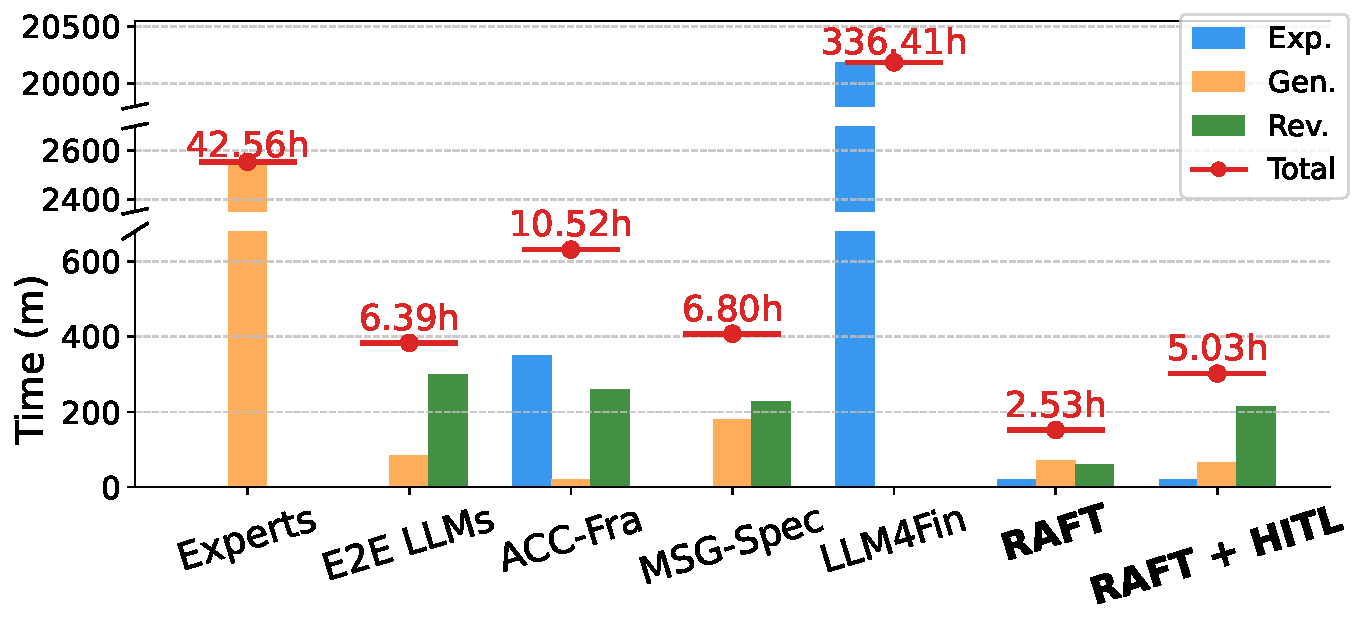
\includegraphics[width=0.60\linewidth]{fig/exp1_time.pdf}
    \caption{Elapsed workflow time across the six financial datasets. Exp., Gen., and Rev.\ denote knowledge explication, test generation, and review or repair.}
    \label{fig:exp1_time}
    \Description{A broken-axis bar chart compares end-to-end time for experts, four baselines, RAFT, and RAFT plus HITL. The measured expert workflow takes 42.56 person-hours; RAFT and its HITL variant take 2.53 and 5.03 hours of elapsed time, respectively. The HITL review requires 7.16 person-hours.}
\end{figure}








\begin{table}[!t]
    \setlength{\tabcolsep}{35pt}
    \caption{Observed per-dataset token usage and provider-billed API cost on the six financial datasets.}
    \label{tab:exp1_token}
    \centering
    \resizebox{\linewidth}{!}{
    \begin{tabular}{|c|c|c|c|}
    \hline
    \textbf{Method} & \textbf{Prompt Tokens} & \textbf{Completion Tokens} & \textbf{API Cost (\$)} \\
    \hline
    \textbf{E2E LLMs} & 115,842 & 1,328,617 & 26.947 \\
    \textbf{MSG-Spec} & 342,517 & 1,685,236 & 35.018 \\
    \textbf{LLM4Fin} & 227,341 & 114,812 & -- \\
    \textbf{\ourtool} & 1,047,286 & 352,043 & 11.463 \\
    \hline
    \end{tabular}
    }
    
\end{table}


Fig.~\ref{fig:exp1_time} reports the elapsed time of each implemented
workflow. Fully automated \ourtool\ completes all six datasets in 2.53 hours.
\ourtool\ + HITL takes 5.03 wall-clock hours: 1.45 hours for its automated stages
and 3.58 hours for concurrent expert review. The review logs record a mean of
10.37 seconds for each of the 1,242 requirement--testability decision pairs for
each expert. Two experts therefore contribute 7.16
person-hours; person-hours are reported separately rather than added to elapsed
time. The measured single-expert workflow requires 42.56 person-hours under the
logged batch-template workflow. We report absolute values, not speedup factors,
because the automated workflows have different execution and review
requirements.





As shown in Table~\ref{tab:exp1_token}, the G-V-R and OCL Cons.\ stages in
Table~\ref{tab:exp3_} contribute 107,734 prompt tokens and 320,059 completion
tokens per dataset. The totals add amortized domain-level knowledge explication
and repeated knowledge injection. Per-request usage and billing records retain
the model identifier, prompt tokens, completion tokens, and charged amount for
GPT-6-Astra, Grok-4.7, and Gemini-3.8-Flash. Aggregating these records by method
and reporting the mean across the six datasets gives 1,047,286 prompt tokens,
352,043 completion tokens, and an actual API charge of \$11.463 per dataset for
\ourtool. The corresponding actual charges for E2E LLMs and MSG-Spec are
\$26.947 and \$35.018,
primarily because \ourtool\ produces substantially fewer completion tokens.
LLM4Fin has no API charge because it is deployed locally; the table therefore
should not be read as a total-cost comparison that includes hardware. All API
figures are observed provider charges; local compute and labor are excluded.


\noindent\textbf{Answer to RQ1.}
\ourtool\ has the highest descriptive result among automated methods
(91.7\% F1, 87.1\% BSC) at an actual API cost of \$11.463 per dataset. The differences favor
\ourtool\ on all six datasets, but no superiority comparison remains
significant after Holm correction; HITL reaches 96.2\% F1 without establishing
equivalence to experts.






\subsection{Experiment II: Ablation Study}
\label{sec:exp2}

\noindent
\textbf{Experimental Design.}
Experiment~II addresses RQ2 through four controlled analyses.
First, an \emph{artifact ablation} compares full \ourtool\
($\mathcal{M}{+}\mathcal{R}{+}\mathcal{T}$) with
(i) $\mathcal{M}{+}\mathcal{R}$, which omits testability constraints and
generates from all formal requirements; (ii) $\mathcal{T}$, which omits the
meta-model and requirements representation and applies testability guidance
directly to regulatory rules; and (iii) \textit{No Knowledge}, which uses no
explicit artifacts.
Here, \textit{No Knowledge} means ``no explicit artifacts''; it does not
remove parametric knowledge from the LLM. The E2E baseline in Experiment~I
instead removes the staged formalization workflow and generates tests directly.

The ablation units follow the dependency chain
$\mathcal{M}\rightarrow\mathcal{R}\rightarrow\mathcal{T}$. In particular,
$\mathcal{R}$ defines its symbols, data dictionary, and grammar over the
entities and relations in $\mathcal{M}$, while $\mathcal{M}$ has no direct
downstream interface and becomes operational only through $\mathcal{R}$.
Consequently, an $\mathcal{M}$-only configuration cannot formalize
requirements. Conversely, a frozen $\mathcal{R}$ generated from $\mathcal{M}$
already encodes its entities and structure, so calling it
``$\mathcal{R}$-only'' would not remove the effect of $\mathcal{M}$; regenerating
$\mathcal{R}$ without $\mathcal{M}$ would change the construction process and
allow the LLM to reconstruct an implicit meta-model. The same issue applies to
$\mathcal{R}{+}\mathcal{T}$. We therefore treat
$\mathcal{M}{+}\mathcal{R}$ as a coupled structural unit and compare only
implemented pipeline configurations. These ablations measure the contribution
of valid knowledge bundles and testability guidance, not independent causal
effects for $\mathcal{M}$ and $\mathcal{R}$.

Second, a \emph{construction-source analysis} tests whether useful meta-level
artifacts can be constructed without external domain documents or historical
tests, and how much the optional corpus improves the resulting workflow.
\ourtool\ w/o Corpus constructs the same three artifacts from the domain/task
description and LLM parametric knowledge. The held-out evaluation regulations
are still supplied in Phase~II as the source of rule-specific semantics.
\textit{Full-Corpus Prompting} supplies the entire construction corpus directly
to the LLM in each generation prompt but does not transform it into explicit
artifacts, while
\ourtool\ w/ Expert Artifacts replaces automatically explicated artifacts with
expert-constructed ones.

Third, a \emph{multi-LLM analysis} contrasts joint use
of GPT-6-Astra, Grok-4.7, and Gemini-3.8-Flash with each backend alone.

Finally, an \emph{end-to-end operator-assignment analysis} compares
all-purification, all-aggregation, the reversed assignment, and \ourtool's
assignment. Each setting restarts Phase~I from the same source inputs and run
seed. After setting-specific consolidation of $\mathcal{M}$, the LLMs
regenerate $\mathcal{R}$ candidates conditioned on that $\mathcal{M}$; after
consolidating $\mathcal{R}$, they likewise regenerate $\mathcal{T}$ candidates.
Phase~II then regenerates the formal requirements and tests. Thus, settings do
not share downstream candidate artifacts whose inputs have changed.

We also vary $N$ and $K$; the $N=2$ result averages all three LLM pairs. The
default operator assignment and $N=3$, $K=2$ are frozen before evaluation; these
variants form a preplanned sensitivity analysis and are not used to choose the
reported default.

Artifact quality is measured against expert-consensus artifacts. Atomic
elements are entities and relations for $\mathcal{M}$; symbols, dictionary
entries, and grammar productions for $\mathcal{R}$; and individual constraints
for $\mathcal{T}$. Two experts independently judge whether normalized elements
are semantically equivalent and reconcile disagreements. These decisions are
used to compute artifact-level Precision and Recall. All four analyses also
report downstream F1 and BSC. The remaining evaluation follows Experiment~I.



\noindent
\textbf{Experimental Results.}
Fig.~\ref{fig:exp2} shows a monotonic loss as guidance is removed. Relative
to full \ourtool, $\mathcal{M}{+}\mathcal{R}$ reduces mean Precision by 33.6\%
and Recall by 19.5\%. The larger Precision loss is consistent with the role of
$\mathcal{T}$: without a testability filter, non-testable rules produce
additional unmatched cases. Retaining only $\mathcal{T}$ causes still larger
relative losses (74.8\% in Precision and 39.6\% in Recall), showing that
testability guidance cannot replace the structural vocabulary and grammar in
$\mathcal{M}$ and $\mathcal{R}$. \textit{No Knowledge} is lowest on every
metric; F1 and BSC follow the same ordering.

\begin{figure*}[!t]
    \centering
    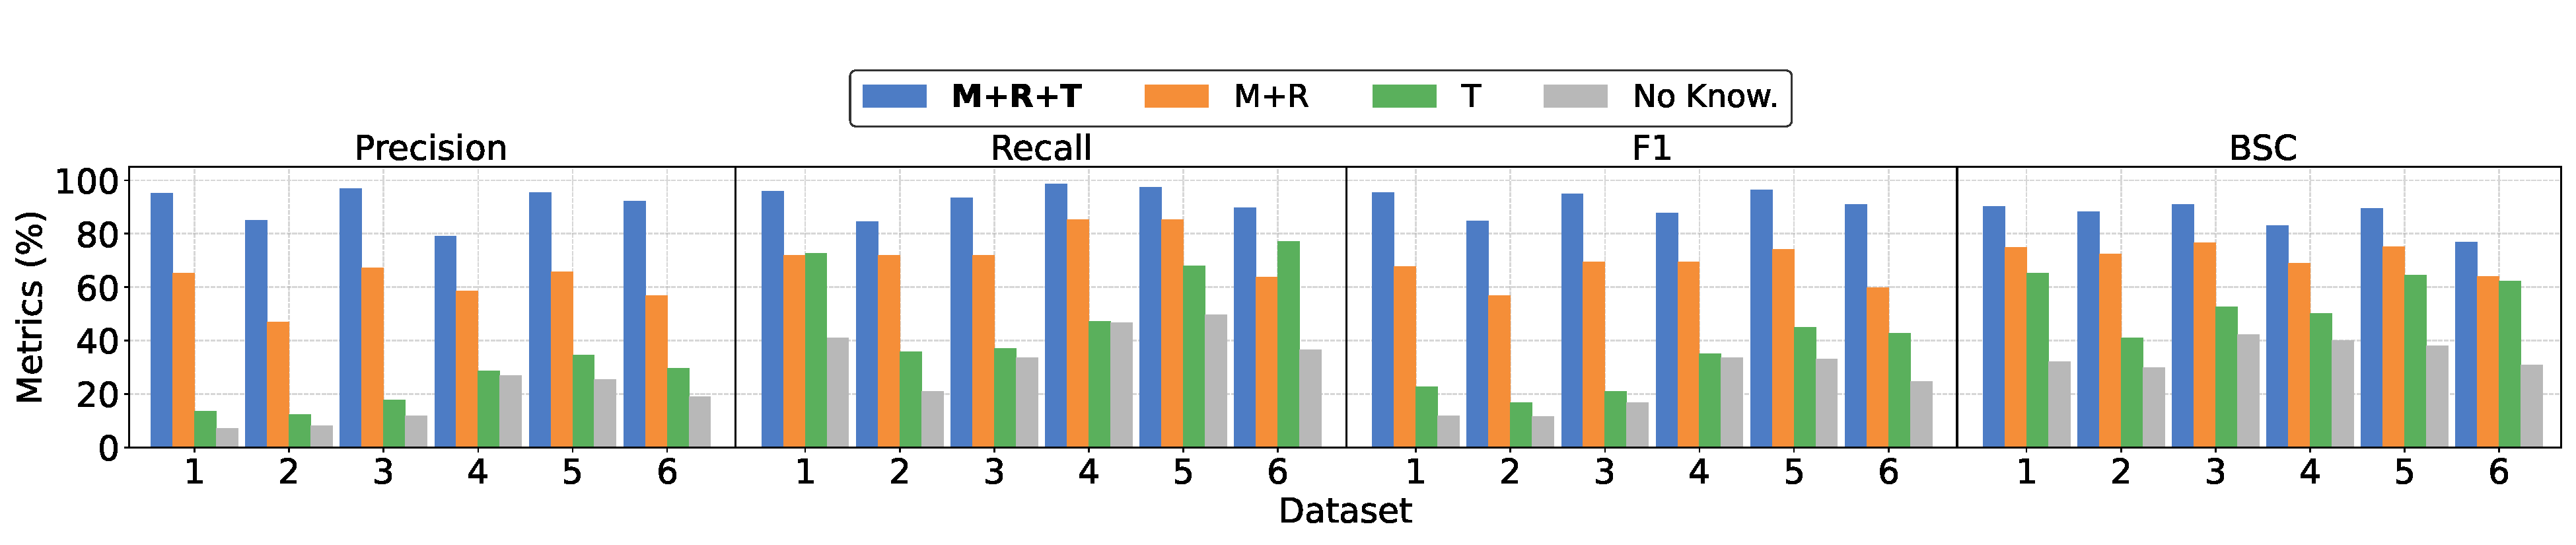
\includegraphics[width=\linewidth]{fig/exp2_all_metrics.pdf}
    \caption{Generated-test impact of valid knowledge bundles. $\mathcal{M}{+}\mathcal{R}$ is coupled because $\mathcal{R}$ is defined over $\mathcal{M}$; ``No Know.'' removes only explicit artifacts.}
    \label{fig:exp2}
    \Description{Four grouped bar charts compare Precision, Recall, F1, and BSC for full RAFT and three knowledge-ablation variants on six datasets. Full RAFT is highest throughout.}
\end{figure*}

\begin{figure*}[!t]
    \centering
    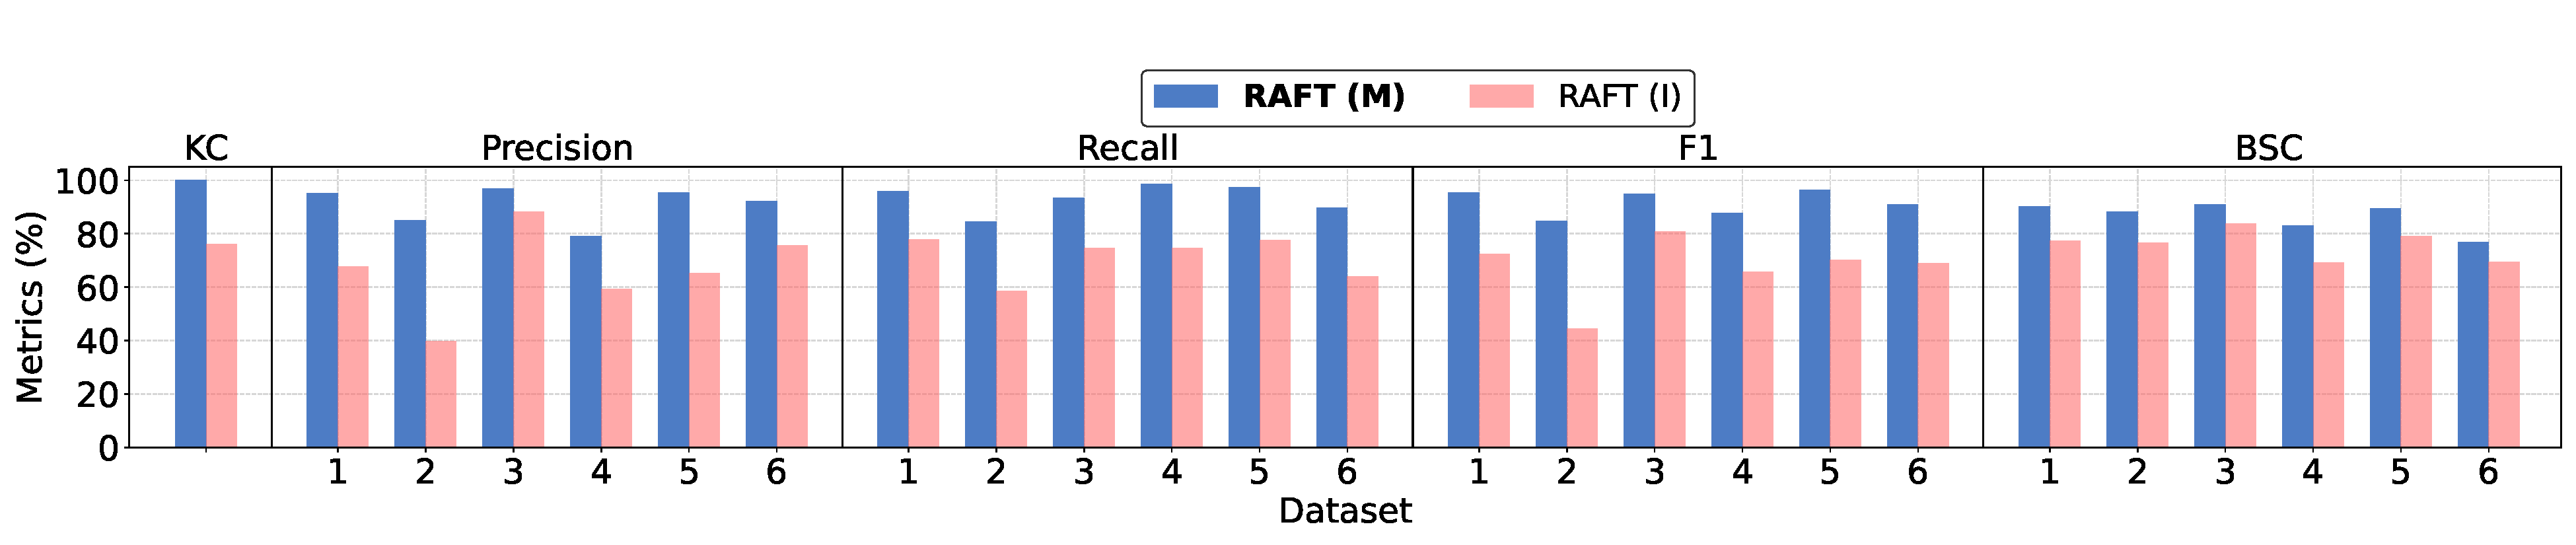
\includegraphics[width=\linewidth]{fig/exp2_2.pdf}
    \caption{Comparison of \ourtool\ using the \strategy\ strategy (\ourtool\ (M)) versus individual LLMs (\ourtool\ (I)). Knowledge coverage (KC) is the percentage of expert-consensus knowledge elements recovered; the remaining measures evaluate generated tests.}
    \label{fig:exp2_2}
    \Description{Grouped bar charts compare multi-LLM and individual-LLM RAFT for knowledge coverage, Precision, Recall, F1, and BSC. The multi-LLM setting is higher in every comparison.}
\end{figure*}

Fig.~\ref{fig:exp2_2} further shows that the individual-LLM variants have
23.9\% lower knowledge coverage, 26.8\% lower F1, and 12.2\% lower BSC on
average than the multi-LLM setting. This result shows the value of
consolidating multiple candidates; the operator analysis below tests whether
the proposed artifact-specific assignment preserves this gain downstream.

\begin{table*}[!t]
    \setlength{\tabcolsep}{5pt}
    \caption{Construction-source analysis on the six financial datasets. Each fidelity or coverage cell reports mean $\pm$ run-level standard deviation; within each run, results are macro-averaged across the six datasets and three LLM backends. Human effort measures the total person-hours required to construct and reconcile the knowledge artifacts and excludes downstream generation time.}
    \label{tab:exp2_source}
    \centering
    \resizebox{\linewidth}{!}{
    \begin{tabular}{lcccrrrrr}
        \toprule
        \textbf{Setting} &
        \textbf{\makecell{Construction\\Corpus}} &
        \textbf{\makecell{Explicit\\Artifacts}} &
        \textbf{Artifact Source} &
        \textbf{\makecell{Human Effort\\(person-h)}} &
        \textbf{Pre. (\%)} &
        \textbf{Rec. (\%)} &
        \textbf{F1 (\%)} &
        \textbf{BSC (\%)} \\
        \midrule
        \ourtool\ w/o Corpus & No & $\mathcal{M}{+}\mathcal{R}{+}\mathcal{T}$ & Multi-LLM & 0 & 82.8 $\pm$ 1.8 & 82.7 $\pm$ 2.1 & 82.7 $\pm$ 2.0 & 78.8 $\pm$ 1.7 \\
        Full-Corpus Prompting & Yes & None & -- & 0 & 62.6 $\pm$ 1.3 & 62.5 $\pm$ 1.2 & 62.5 $\pm$ 1.3 & 58.5 $\pm$ 1.2 \\
        \ourtool & Yes & $\mathcal{M}{+}\mathcal{R}{+}\mathcal{T}$ & Multi-LLM & 0 & 90.6 $\pm$ 6.7 & 93.0 $\pm$ 3.8 & 91.7 $\pm$ 4.3 & 87.1 $\pm$ 6.5 \\
        \ourtool\ w/ Expert Artifacts & Yes & $\mathcal{M}{+}\mathcal{R}{+}\mathcal{T}$ & Experts & 24.37 & 94.0 $\pm$ 3.0 & 93.9 $\pm$ 3.4 & 94.0 $\pm$ 3.2 & 91.2 $\pm$ 3.8 \\
        \bottomrule
    \end{tabular}
    }
\end{table*}

Table~\ref{tab:exp2_source} supports three controlled comparisons.
Without any construction corpus, \ourtool\ still reaches 82.7\% F1 and 78.8\%
BSC, retaining 90.2\% and 90.5\% of the full method's scores after all document
and historical-test cues are removed from artifact construction. This is
operational evidence that LLM parametric knowledge can induce useful
meta-level artifacts without an external construction corpus; it does not
imply that rule-specific semantics are recovered without reading the held-out
regulations in Phase~II. Adding the corpus raises F1 by 9.0 points and BSC by
8.3 points by providing additional evidence about expected content,
abstraction, terminology, and format.

\textit{Full-Corpus Prompting}
has access to the same corpus as \ourtool\ but trails it by 29.2 F1 points and
28.6 BSC points, indicating that transforming available knowledge into
structured artifacts contributes beyond placing the same corpus directly in
the generation context.

Expert-constructed artifacts add
only 2.3 F1 points and 4.1 BSC points over automatic explication but require 24.37
person-hours. Thus, the automatically explicated artifacts approach the
reference-case fidelity achieved by expert-constructed artifacts while
eliminating manual \emph{artifact-construction} effort;
this does not include evaluation or optional HITL review.

\begin{table*}[!t]
    \setlength{\tabcolsep}{10pt}
    \caption{End-to-end consolidation-operator assignment and hyperparameter sensitivity. Pur.\ and Agg.\ denote $K$-consensus purification and union-based aggregation, respectively. Artifact-quality cells report Precision/Recall (\%) against the expert-consensus artifacts; downstream F1 and BSC report mean $\pm$ run-level standard deviation. The $N=2$ setting is averaged over all three LLM pairs.}
    \label{tab:exp2_strategy}
    \centering
    \resizebox{\linewidth}{!}{
    \begin{tabular}{lccccccccrr}
        \toprule
        \textbf{Setting} &
        \textbf{$N$} & \textbf{$K$} &
        \textbf{$\mathcal{M}$} &
        \textbf{$\mathcal{R}$} &
        \textbf{$\mathcal{T}$} &
        \textbf{\makecell{$\mathcal{M}$ P/R\\(\%)}} &
        \textbf{\makecell{$\mathcal{R}$ P/R\\(\%)}} &
        \textbf{\makecell{$\mathcal{T}$ P/R\\(\%)}} &
        \textbf{F1 (\%)} &
        \textbf{BSC (\%)} \\
        \midrule
        All Purification & 3 & 2 & Pur. & Pur. & Pur. & 98.9/93.0 & 100.0/66.7 & 100.0/66.0 & 84.4 $\pm$ 2.8 & 78.6 $\pm$ 1.1 \\
        All Aggregation & 3 & -- & Agg. & Agg. & Agg. & 83.1/98.0 & 73.6/94.7 & 68.1/96.0 & 87.1 $\pm$ 2.7 & 79.9 $\pm$ 1.7 \\
        Reversed & 3 & 2 & Agg. & Pur. & Pur. & 83.1/98.0 & 100.0/71.3 & 100.0/69.0 & 85.2 $\pm$ 2.8 & 78.7 $\pm$ 2.6 \\
        \ourtool & 3 & 2 & Pur. & Agg. & Agg. & 98.9/93.0 & 83.6/92.0 & 72.7/96.0 & 91.7 $\pm$ 4.3 & 87.1 $\pm$ 6.5 \\
        \midrule
        \ourtool\ (Pairwise) & 2 & 2 & Pur. & Agg. & Agg. & 99.6/87.0 & 88.1/85.8 & 78.6/81.0 & 86.0 $\pm$ 2.1 & 79.3 $\pm$ 2.5 \\
        \ourtool\ (Strict) & 3 & 3 & Pur. & Agg. & Agg. & 100.0/84.0 & 83.4/90.7 & 71.4/90.0 & 87.2 $\pm$ 1.5 & 79.4 $\pm$ 1.2 \\
        \bottomrule
    \end{tabular}
    }
\end{table*}

Table~\ref{tab:exp2_strategy} shows the same trade-off at artifact and pipeline
levels. All Purification raises precision but reduces
$\mathcal{R}$/$\mathcal{T}$ recall to 66.7\%/66.0\%, yielding 84.4\% F1. All
Aggregation retains 94.7\%/96.0\% recall but propagates structural noise,
yielding 87.1\% F1; Reversed reaches 85.2\%. \ourtool's assignment retains
98.9\% $\mathcal{M}$ precision and 92.0\%/96.0\%
$\mathcal{R}$/$\mathcal{T}$ recall, producing the highest F1 (91.7\%) and BSC
(87.1\%). Two LLMs and unanimity lower downstream F1 to 86.0\% and 87.2\%,
respectively; these variants were preplanned and did not tune the default.

\noindent\textbf{Answer to RQ2.}
Corpus-free LLM-derived artifacts provide a strong starting point (82.7\% F1);
the corpus-supported workflow reaches 91.7\%. Purifying $\mathcal{M}$ and
aggregating $\mathcal{R}$ and $\mathcal{T}$ yields 4.6--7.3 more F1 points than
the alternative operator assignments after regenerating their dependent
artifacts and tests. Evaluation regulations remain the source of rule-specific semantics.
The ablation evaluates coupled $\mathcal{M}{+}\mathcal{R}$ and $\mathcal{T}$
rather than individual $\mathcal{M}$ or $\mathcal{R}$ effects.





\subsection{Experiment III: Step-Level Performance}
\label{sec:exp3}

\noindent
\textbf{Experimental Design.}
Experiment~III localizes the residual end-to-end errors observed in
Experiment~I. On the same six datasets, we compare one-shot requirements
generation (G Only) with up to three G-V-R repair iterations, and compare
natural-language (NL Cons.) with OCL-style testability criteria (OCL Cons.).
The latter are deterministic renderings of the same frozen five predicates,
with identical scope, polarity, exceptions, labels, and order. Two experts
verify their semantic correspondence; all other inputs and settings remain
fixed.

\noindent\textbf{Gold-Standard Construction.}
Before any run, two experts independently derive requirements and testability
labels from the source rules under a fixed guide and without model outputs.
They encode atomic obligations, conditions, exceptions, and outcomes as
\textit{KEY-OP-VALUE} with evidence and
\textit{Status}/\textit{ResultStatus}. Disagreements are resolved against the
source, followed by an omission check; the resulting versioned gold set is
frozen, hidden, and reused unchanged. The one-to-many rule mapping explains
Table~\ref{tab:exp1_dataset}. Requirements and labeled testability decisions
use the same maximum one-to-one set matching: unmatched generated items are
FPs, unmatched gold items are FNs, and a field or label mismatch leaves both
items unmatched, yielding one FP and one FN. Time and prompt/completion tokens
are also reported.

\begin{table}[!t]
    \setlength{\tabcolsep}{15pt}
    \caption{Step-level evaluation against the expert-constructed gold standard frozen before any model variant is run. The same gold set is used for every variant. Fidelity and classification metrics are macro-averaged across the six financial datasets; time and tokens are totals for processing all six.}
    \label{tab:exp3_}
    \centering
    \resizebox{\linewidth}{!}{
    \begin{tabular}{|c|c|ccc|c|cc|}
    \hline
    \textbf{Step} & \textbf{Variant} & \textbf{Pre. (\%)} & \textbf{Rec. (\%)} & \textbf{F1 (\%)} & \textbf{Time (m)} & \textbf{PTok} & \textbf{CTok} \\
        \hline
        \multirow{2}{*}{\makecell{\textbf{Requirements}\\\textbf{Generation}}} & G Only & 79.6 & 75.3 & 77.4 & 12.5 & 68,214 & 318,146\\
        \cline{2-8}
         & G-V-R & 91.6 & 87.7 & 89.0 & 34.9 & 210,247 & 982,237\\
        \hline
        \multirow{2}{*}{\makecell{\textbf{Testability}\\\textbf{Determination}}} & NL Cons. & 69.4 & 77.1 & 73.0 & 15.8 & 318,104 & 1,028,132\\
        \cline{2-8}
         & OCL Cons. & 96.2 & 95.5 & 95.8 & 14.6 & 436,159 & 938,117\\
        \hline
    \end{tabular}
    }
    \vspace{-2mm}
\end{table}


\noindent
\textbf{Experimental Results.}
Table~\ref{tab:exp3_} shows that G-V-R raises requirements-generation F1 from
77.4\% to 89.0\% (+11.6 points), primarily through a 12.0-point precision
gain. The repair loop adds 22.4 minutes, 142,033 prompt tokens, and 664,091
completion tokens over all six datasets. This is a measurable trade-off rather
than a free gain: G-V-R improves correctness, but omitted, incorrect, and
redundant elements remain and can propagate to final tests.

For testability determination, OCL Cons. raises F1 from 73.0\% to 95.8\%
(+22.8 points) while taking 1.2 fewer minutes. It uses 118,055 more prompt tokens
but 90,015 fewer completion tokens, leaving total token usage comparable. The
improvement in both Precision and Recall indicates that OCL-style serialization
presents the same scopes and predicates more consistently to the model than
their natural-language rendering.

Some errors are inherited from imperfect input requirements. The reported
testability score should therefore be interpreted as conditional on the
correctness of its input requirement.

% Since neither step is error-free, \ourtool\ supports a human-in-the-loop where experts correct the intermediate results. 
% As shown in Experiment~I, this intervention pushes \ourtool\ past expert-level performance with even less effort.




\noindent\textbf{Answer to RQ3.}
G-V-R improves requirements-generation F1 by 11.6 points to 89.0\%.
Representing the same testability predicates in OCL-style rather than
natural-language form improves testability F1 by 22.8 points to 95.8\%.



\subsection{Experiment IV: Sensitivity to LLM Backbone}
\label{sec:exp4}

\noindent
\textbf{Experimental Design.}
Experiment~IV addresses RQ4 by replacing the default backends with 11
open-weight LLMs spanning 2B--1.04T total parameters (Table~\ref{tab:exp4_llm}).
We report provider-stated total parameter counts only to describe and order the
tested backbones. The models also differ in architecture, training data, and
context length, so this experiment measures practical sensitivity to backbone
choice rather than the causal effect of parameter count or a scaling threshold.

Because each setting contains one LLM, that LLM independently explicates three
candidate versions of each artifact; \strategy\ then consolidates them before
the same LLM generates tests. The paired E2E baseline uses that model to
generate tests directly without \ourtool, while retaining the same evaluation
documents, output fields, matcher, and run protocol. On the six financial
datasets, we repeat each complete configuration three times and report mean F1;
the run-level minimum and maximum indicate variability. These models are
accessed through the OpenRouter endpoints listed in the replication package,
rather than a common local inference stack, so runtime and quantization are not
controlled or compared.

\begin{table}[!t]
    \setlength{\tabcolsep}{18pt}
    \caption{Open-weight LLMs used in the backbone-sensitivity analysis. Parameter counts are provider-reported total parameters used for descriptive ordering only; a dash indicates an undisclosed training cutoff.}
    \label{tab:exp4_llm}
    \centering
    \resizebox{\linewidth}{!}{
    \begin{tabular}{|c|c|c|c|c|}
    \hline
    \textbf{LLM} & \textbf{Total Params} & \textbf{Provider} & \textbf{Training Cutoff} & \textbf{Context Length} \\
        \hline
        Qwen3.5-2B \cite{qwen35_2b} & 2B & Alibaba & -- & 256K \\
        Gemma3-4B \cite{kamath2025gemma} & 4B & Google & 2024.08 & 128K \\
        Qwen3-4B \cite{yang2025qwen3} & 4B & Alibaba & - & 32K \\
        Gemma3-12B \cite{kamath2025gemma} & 12B & Google & 2024.08 & 128K \\
        GPT-OSS-20B \cite{agarwal2025gpt} & 21B & OpenAI & 2024.06 & 128K \\
        Gemma3-27B \cite{kamath2025gemma} & 27B & Google & 2024.08 & 128K \\
        Llama3.3-70B \cite{llama33} & 70B & Meta & 2023.12 & 128K \\
        GPT-OSS-120B \cite{agarwal2025gpt} & 117B & OpenAI & 2024.06 & 128K \\
        GLM4.5 \cite{zeng2025glm} & 355B & Zhipu AI & -- & 128K \\
        Llama3.1-405B \cite{grattafiori2024llama} & 405B & Meta & 2023.12 & 128K \\
        KimiK2 \cite{team2025kimi} & 1.04T & Moonshot AI & - & 256K \\
        \hline
    \end{tabular}
    }
\end{table}

\begin{figure}[!t]
    \centering
    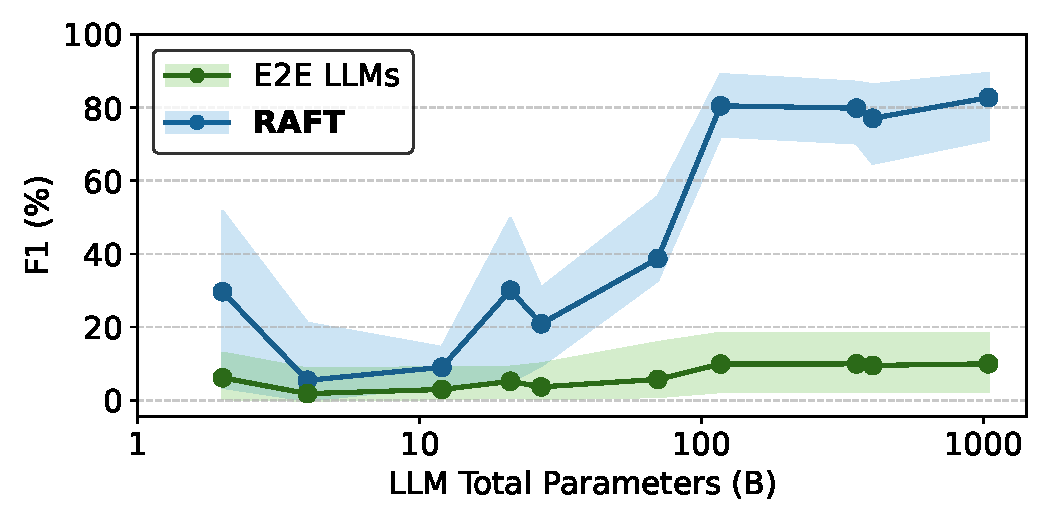
\includegraphics[width=0.6\linewidth]{fig/exp4.pdf}
    \caption{F1 for the tested LLM backbones, ordered by provider-reported total parameter count, for \ourtool\ and direct E2E generation. Lines denote three-run means and shaded regions denote run-level minima and maxima; the ordering does not identify a causal parameter-count effect.}
    \label{fig:exp4}
    \Description{A log-scale line chart orders tested backbones by provider-reported total parameter count. RAFT F1 varies substantially across models, while direct E2E generation remains near or below 10 percent for most models.}
\end{figure}


\noindent
\textbf{Experimental Results.}
Fig.~\ref{fig:exp4} reveals strong backbone dependence. Among the tested
models, those below 100B total parameters vary from near-zero to 38.7\% mean F1,
while the four selected models above 100B cluster at
76\%--83\%. This sampled pattern establishes neither a 100B threshold nor a
causal scaling relationship, and run ranges vary across backbones.

\ourtool\ exceeds the paired E2E baseline for 10 of the 11 models. The gap
varies across backbones, while direct generation remains near or below 10\% F1
for most tested models. Non-monotonic results among similarly sized models
reinforce that parameter count, architecture, training data, context length, and
provider runtime remain confounded.

Within-backbone gaps are more informative than cross-backbone ordering. Each
pair fixes the backbone, documents, schema, and matcher, but not calls or
tokens; it therefore evaluates the complete staged workflow rather than an
isolated artifact effect.


\noindent\textbf{Answer to RQ4.}
\ourtool\ improves over direct generation for 10 of 11 models, but remains
backbone-dependent; the experiment establishes neither a parameter threshold
nor a causal scaling effect.















\subsection{Experiment V: Cross-Domain Workflow Re-instantiation}
\label{sec:exp5}

\noindent
\textbf{Experimental Design.}
Experiment~V uses three road-traffic and two power-system datasets
(Table~\ref{tab:exp5_dataset}). Each pairs a cited official document with
pre-existing industry-authored reference cases, created independently of
\ourtool, source-checked, and frozen before evaluation. We retain the cited
language and edition and normalize only field names. Each family builds a
separate corpus; prompts, $N=3$, $K=2$, downstream procedure, metrics, schemas,
and operators remain fixed, and no financial artifact is reused.

\begin{table}[!t]
    \setlength{\tabcolsep}{15pt}
    \caption{Details of the five road-traffic and power-system evaluation datasets in Experiment V.}
    \label{tab:exp5_dataset}
    \centering
    \resizebox{\linewidth}{!}{
    \begin{tabular}{|c|c|p{5cm}|c|c|c|}
    \hline
    \textbf{Dataset} & \textbf{Domain} & \textbf{Document} & \textbf{\# Rule} & \textbf{\# Req.} & \textbf{\# TC} \\
        \hline
        \multirow{1}{*}{7} & \multirow{3}{*}{Road Traffic} & 2025 New Jersey Driver Manual \cite{dataset7} & \multirow{1}{*}{47} & \multirow{1}{*}{427} & \multirow{1}{*}{1570} \\
        \cline{1-1}\cline{3-6}
        \multirow{1}{*}{8} & & Road Traffic Safety Law of PRC \cite{dataset8} & \multirow{1}{*}{171} & \multirow{1}{*}{613} & \multirow{1}{*}{2124} \\
        \cline{1-1}\cline{3-6}
        \multirow{1}{*}{9} & & Cambodian Road Traffic Law \cite{dataset9} & \multirow{1}{*}{93} & \multirow{1}{*}{808} & \multirow{1}{*}{3132} \\
        \hline
        \multirow{1}{*}{10} & \multirow{2}{*}{Power} & EN 50549-1:2019 \cite{dataset10} & \multirow{1}{*}{75} & \multirow{1}{*}{362} & \multirow{1}{*}{703} \\
        \cline{1-1}\cline{3-6}
        \multirow{1}{*}{11} & & GB/T 19964-2024 \cite{dataset11} & \multirow{1}{*}{189} & \multirow{1}{*}{195} & \multirow{1}{*}{1311} \\
        \hline
    \end{tabular}
    }
\end{table}

\begin{figure}[!t]
    \centering
    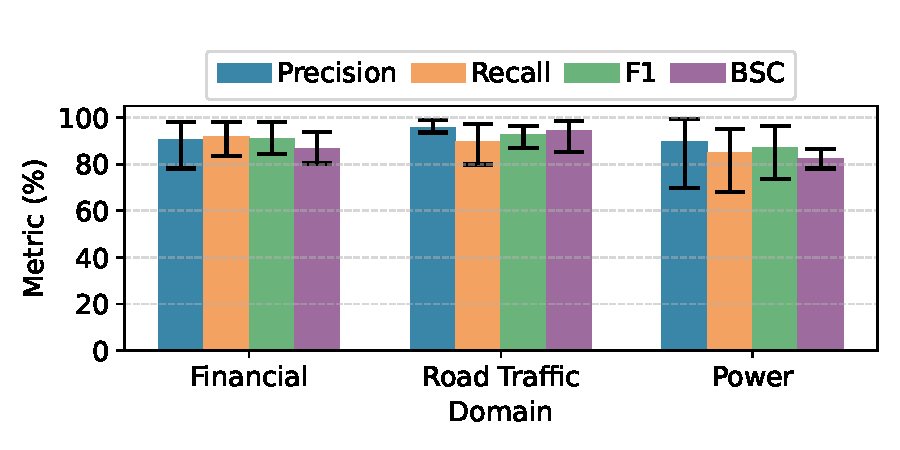
\includegraphics[width=0.5\linewidth]{fig/exp3.pdf}
    \caption{Family-level metric means; error bars show minimum and maximum dataset means.}
    \label{fig:exp5}
    \Description{A grouped bar chart shows Precision, Recall, F1, and BSC in the financial, road-traffic, and power-system document domains, with the power-system means lower and more variable.}
    \vspace{-2mm}
\end{figure}

\noindent
\textbf{Experimental Results.}
Road-traffic F1/BSC is 92.7\%/94.3\%, versus 91.7\%/87.1\% in finance;
power performance is 87.2\%/82.3\% (Fig.~\ref{fig:exp5}). Without domain
baselines, these differences are descriptive. Relative to finance, road traffic
is 1.0 F1 and 7.2 BSC points higher, whereas power is 4.5 F1 and 4.8 BSC points
lower. The error-bar ranges further show variation among documents within each
family; five non-financial datasets cannot establish broad domain superiority.

\noindent\textbf{Answer to RQ5.}
The workflow transfers after domain-specific re-instantiation while retaining
its artifact types and downstream protocol; the evidence does not establish
zero-shot portability.




\subsection{Threats to Validity}

\noindent
\textbf{Internal Validity.}
LLM stochasticity and baseline reimplementation remain; matched E2E runs,
ablations, paired operator settings with common source inputs and run seeds,
and common NL/OCL predicates reduce confounding. Each operator setting
regenerates dependent artifacts and tests, so its comparison is end-to-end.

\noindent
\textbf{Construct Validity.}
Incomplete reference cases and matcher errors mean F1/BSC measure fidelity, not
exhaustive validity or fault detection. Corpus-free does not remove parametric
knowledge; $\mathcal{M}{+}\mathcal{R}$ is coupled, and expert groups differ.
Residual subjectivity remains despite over 90\% initial agreement and
source-grounded reconciliation.

\noindent
\textbf{External Validity.}
Only five of 11 documents are outside finance, all reference cases are industrial, and
no domain baselines exist; evidence is limited to the evaluated documents.

\noindent
\textbf{Conclusion Validity.}
Six pairs provide limited power; corrected tests establish neither significance
nor expert equivalence. Experiment~IV establishes sensitivity, not a parameter
threshold or causal scaling.







% \subsection{Experiment IV: Impact of LLMs}

% \noindent
% \textbf{Experimental Design.}
% This experiment investigates how the capability of the underlying LLM affects knowledge extraction for constructing the meta-model and testable requirements representations. We approximate model capability by parameter size, evaluating 12 advanced LLMs with 2B-1T parameters under two settings: (1) each LLM performs the task individually, and (2) LLMs are grouped into four sets of three similarly sized models for aggregation. We then compare the completeness of the constructed meta-model and requirements representations, where \emph{completeness} is the percentage of correctly extracted elements, symbols, syntax, and testability components relative to the methodology in the main text. Model details are provided in Appendix \ref{sec:app:exp3}.


% \begin{figure}
%     \centering
%     \begin{subfigure}{0.235\textwidth}
%         \centering
%         \includegraphics[width=\textwidth]{fig/exp3_metamodel_completion.png}
%         \caption{Meta-Model}
%         \label{fig:exp3_metamodel}
%     \end{subfigure}
%     \begin{subfigure}{0.235\textwidth}
%         \centering
%         \includegraphics[width=\textwidth]{fig/exp3_representation_completion.png}
%         \caption{Req. Representation}
%         \label{fig:exp3_representation}
%     \end{subfigure}
%     \caption{Impact of LLM parameter size on the completeness of extracted domain knowledge.}
%     \label{fig:exp3}
% \end{figure}


% \noindent
% \textbf{Experimental Result.}
% The evaluation results are shown in Figure \ref{fig:exp3}. As the number of parameters increases, the completeness of both the meta-model and requirements representation shows a clear upward trend, indicating that stronger LLMs produce higher quality knowledge extraction. Our multi-LLM aggregation approach achieves over 90\% completeness with LLMs exceeding 100B parameters, establishing a practical lower bound for our method. In contrast, individual LLMs follow a similar trend but exhibit greater variability, reflecting the influence of randomness. Across all parameter settings, the multi-LLM aggregation consistently outperforms individual LLMs, underscoring the effectiveness of aggregation.

% \noindent
% \textbf{Conclusion:}
% Stronger LLMs consistently produce higher-quality knowledge, and our approach achieves over 90\% completeness with a lower bound of LLMs with 100B parameters.


















% \subsection{Experiment IV: Accuracy of Our Testable Requirements Generation}
% \label{sec:exp4}



% \begin{table}
%     \setlength{\tabcolsep}{3pt}
%     \caption{The quality of generated structured requirements of our approach using different LLMs.}
%     \label{tab:exp4_req}
%     \centering
%     \resizebox{\linewidth}{!}{
%     \begin{tabular}{|c|ccccc|ccc|}
%     \hline
%     \multirow{2}{*}{\textbf{O. LLM}} & \multicolumn{5}{c|}{\textbf{Token-Wise}} & \multicolumn{3}{c|}{\textbf{Word-Wise}} \\
%     \cline{2-9}
%      & \textbf{Pre.} & \textbf{Rec.} & \textbf{F1} & \textbf{BLEU} & \textbf{Rouge} & \textbf{Pre.} & \textbf{Rec.} & \textbf{F1} \\
%     \hline
%     GPT-5 & 80.9 & 72.3 & 75.0 & 44.8 & 73.9 & 75.6 & 66.0 & 69.0 \\
%     Grok-4 & 89.5 & 84.3 & 86.0 & 70.5 & 86.0 & 87.8 & 81.4 & 83.6 \\
%     \rowcolor{red!10} DeepSeek-R1 & 91.6 & 87.7 & 89.0 & 76.8 & 89.9 & 89.8 & 85.3 & 86.8 \\
%     \hline
%     \end{tabular}
%     }
% \end{table}


% \begin{table}
%     \setlength{\tabcolsep}{3pt}
%     \caption{Comparison of the accuracy of testability determination of our approach using different LLMs.}
%     \label{tab:exp4_test}
%     \centering
%     \resizebox{\linewidth}{!}{
%     \begin{tabular}{|c|c|c|>{\columncolor{red!10}}c|}
%     \hline
%     \textbf{O. LLM} & \textbf{NL only 1-step} & \textbf{NL+Req. 1-step} & \textbf{NL+Req. 5-step} \\
%     \hline
%     GPT-5 & 59.6 & 72.9 & 82.1 \\
%     Grok-4 & 63.8 & 74.3 & 89.5 \\
%     DeepSeek-R1 & 55.5 & 67.0 & 91.3 \\
%     \hline
%     \end{tabular}
%     }
% \end{table}

% \noindent
% \textbf{Experiment Design.}
% We evaluate the performance of structured requirements generation and testability determination on the 19 financial regulatory documents. Based on the financial metamodel and requirements representation, structured requirements are generated by the three LLMs and compared against manually constructed ground truth. The quality is evaluated using token-level metrics (Precision, Recall, F1, BLEU \cite{papineni2002bleu}, and ROUGE \cite{lin2004rouge}) and word-level metrics (precision, recall, and F1). We further assess downstream testability determination under three settings: (1) using natural language only; (2) using natural language with structured requirements and evaluating all criteria in a single step; and (3) using natural language with structured requirements in a five-step process, where each step evaluates one testability criterion. Precision, Recall, and F1 are reported relative to the ground-truth labels.

% \noindent
% \textbf{Experimental Result.}
% As shown in Table~\ref{tab:exp4_req}, our approach achieves consistently high accuracy in generating structured requirements across different LLMs, as reflected by strong token-level and word-level evaluation metrics. Among the evaluated models, DeepSeek-R1 attains the highest overall performance, indicating more accurate and stable structured requirements generation. 
% Table~\ref{tab:exp4_test} shows that using structured requirements leads to more accurate testability determination than relying on natural-language rules alone. In addition, the multi-step determination strategy consistently outperforms the one-step setting across all LLMs, suggesting that decomposing testability assessment into finer-grained steps yields more reliable results.

% \noindent
% \textbf{Conclusion:}
% Our approach is able to generate high-quality, testable structured requirements, providing a solid foundation for subsequent test generation.
